\chapter{Results}
\label{chap:results}
As mentioned in the previous chapter, for evaluating the performance of the INTERP method I analyzed its performance on several types of graphs, namely cyclic graphs, 3-regular graphs and weighted 3-regular graphs. Additionally, graphs from the Erd\"os-R\'enyi ensemble were investigated with edge probabilities 0.5, and 0.75. As a figure of merit of the performance of QAOA approaches, I used the following quantity, as introduced in \cite{ZWCPL18}
\begin{equation}
	r = \frac{F_p(\gambe)}{C_{\max}}
\end{equation}
where $C_{\max}$ is the actual optimum. I will refer to the quantity $1-r$ as the \emph{fractional error}. As the outcome of Goemans-Williamson is inherently stochastic, I introduce the following quantity to compare the Goemans-Williamson on an equal footing as QAOA
\begin{equation}
	r_{GW}(k) = \frac{\frac{1}{k}\sum_i^kC_{GW,i}}{C_{\max}}
\end{equation}
where I take the average outcome of $k$ samples of $C_{GW}$. In the rest of this chapter I consider $k=10$.

The results from this chapter were obtained using the pyQuil INTERP method \cite{pyQuil-INTERP}, or simply called INTERP, unless stated otherwise. The BFGS optimizer was used for finding the locally optimal parameters $\gambe$, and by iteratively incrementing $p$ using INTERP starting from $p=1$ with parameters $(\gamma_0, \beta_0) = (0.8, 0.35)$. Degeneracies from time reversal symmetry $F_p(\gambe) = F_p(-\vec{\gamma},-\vec{\beta})$ were removed by taking $(\vec{\gamma},\vec{\beta})' = (-\vec{\gamma},-\vec{\beta})$ when $\gamma_i,\beta_i < 0$ for all $i$. Remarkably, for almost all sets of parameters found using INTERP, either all or no angles were found to be negative.

In the appendices the data is presented in more detail. This includes the parameter patterns in Appendix \ref{appendix:patterns}, the runtime of simulating the algorithm in Appendix \ref{appendix:runtime}, and the dependence of the fractional error on $p$ in Appendix \ref{appendix:fractional-error}.

\section{3-regular graphs}

The figure of merit $r$ as well as the fractional error, for 25 random instances of unweighted 3-regular graphs with 12 nodes, are plotted in Figure \ref{fig:Fp 3-regular 12-nodal}. Note that the expectation value $F_p$ asymptotically approaches the optimal objective value as we see that $r$ approaches 1 asymptotically. Results for the other graphs are included in Appendix \ref{appendix:fractional-error}.

\begin{figure}[H]
	\centering
	\begin{subfigure}[t]{0.48\textwidth}
		\centering
		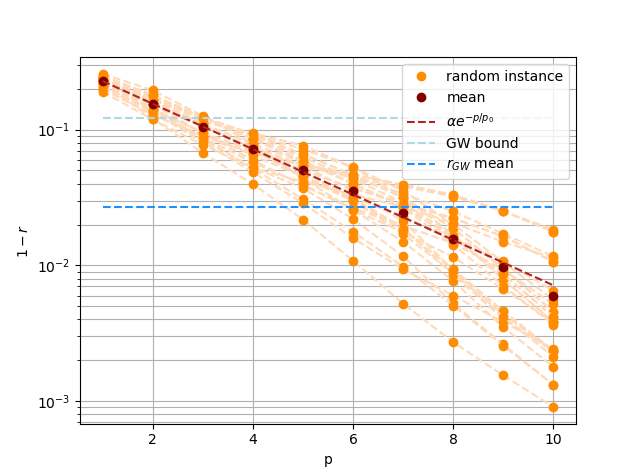
\includegraphics[width=\textwidth]{figures/interp/FOM_12_high_p.png}
		\caption{Fractional error $1-r$}
	\end{subfigure}
	\begin{subfigure}[t]{0.48\textwidth}
		\centering
		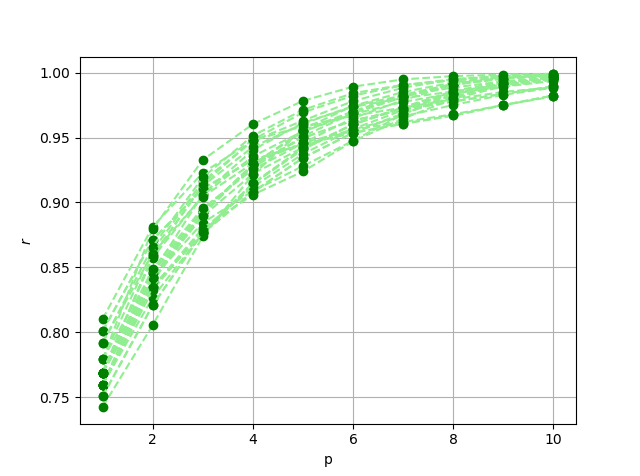
\includegraphics[width=\textwidth]{figures/interp/r_3-regular_12-nodal.png}
		\caption{Figure of merit $r$}
	\end{subfigure}%
	\caption{(a) The fractional error $1-r$ for the various randomly generated instances. A fit is included of the form $ae^{-p/p_0}$ where $\alpha = 0.334 \pm 0.003$ and $p_0 = 2.60 \pm 0.03$. (b) $r$ values after optimization for 25 instances of 12 nodal 3-regular graphs at various depths $p =  1, ... 10$. The angles were obtained by running the Grove QAOA method with the BFGS optimizer, by iteratively incrementing $p$ using INTERP starting from $(\gamma, \beta) = (0.8, 0.35)$.}
	\label{fig:Fp 3-regular 12-nodal}
\end{figure}

In Figure \ref{fig:pattern 3-regular 12-nodal} the patterns of (local) optimal parameters found with the pyQuil INTERP method.
\begin{figure}[H]
	\centering
	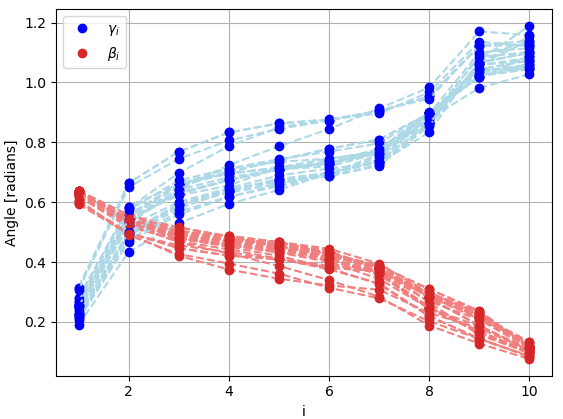
\includegraphics[width=0.5\textwidth]{figures/interp/pattern_3-regular_12-nodal.png}
	\caption{Patterns of the angles $\gambe$ for 25 instances of 12 nodal 3-regular graphs at depth $p=10$.}
	\label{fig:pattern 3-regular 12-nodal}
\end{figure}

These patterns are very reminiscent of the results found in earlier research \cite{Crooks18,ZWCPL18} in Figures \ref{fig:patterns-crooks} and \ref{fig:patterns-zhou} respectively. Not only does the monotonicity of the patterns coincide, the scaling is also very similar to both, taking the factor 2 in the mixer Hamiltonian into account from \cite{Crooks18}.  In Appendix \ref{appendix:patterns} the patterns are shown for different graph sizes $n$ and different classes of graphs. The monotonic patterns seem to be ubiquitous over the different classes of graphs, but there are certainly differences to be seen between the classes. Notable differences include the spread of the patterns for weighted graphs. For unweighted graphs the found parameters for different instances seem to concentrate. Moreover, the range of the patterns differs between the classes. For Erd\"os-R\'enyi graphs $\gamma$ typically varies from $\gamma_1 \approx 0.2$ to $\gamma_p \approx 0.7$ while for 3-regular unweighted graphs we typically find the $\gamma$-parameter ranging from $\gamma_1 \approx 0.4$ to $\gamma_p \approx 1$ and for 3-regular weighted graphs $\gamma_1 \approx 0.6$ to $\gamma_p \approx 1.6$.

In Figure \ref{fig:fom-exp-fit} the relation between $p$ and $r$ for weighted and unweighted 3-regular graphs is shown. As can be seen, for unweighted graphs the fractional error on average decreases exponentially with $p$. For weighted graphs we see a similar pattern, but for this class the fractional error decreases exponentially with the square root of $p$. Similar relations were found in \cite{ZWCPL18} for a similar method to INTERP, namely FOURIER.

\begin{figure}[H]
	\centering
	\begin{subfigure}[t]{0.65\textwidth}
		\centering
		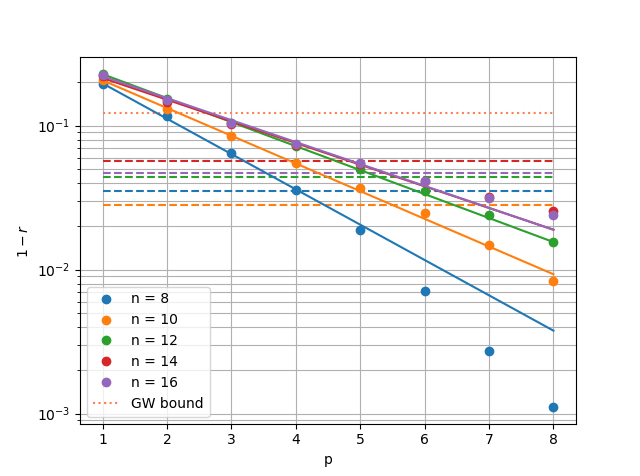
\includegraphics[width=\textwidth]{figures/interp/FOM_(unweighted)/system-size_unweighted_exp.png}
		\captionsetup{justification=centering}
		\caption{Unweighted 3-regular graphs}
	\end{subfigure}
	\\
	\centering
	\begin{subfigure}[t]{0.65\textwidth}
		\centering
		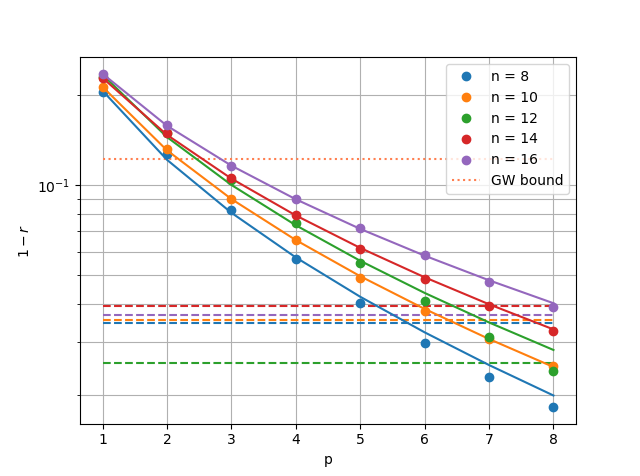
\includegraphics[width=\textwidth]{figures/interp/FOM_(weighted)/SQR/system-size_sqr.png}
		\captionsetup{justification=centering}
		\caption{Weighted 3-regular graphs}
	\end{subfigure}
	\caption{Dependence of $r$ on $n$ on 20 randomly generated unweighted 3-regular (a) and 20 randomly generated weighted 3-regular graphs (b) both using INTERP. For the unweighted graphs the model function $ae^{-p/p_0}$ was used, for the weighted graphs the model function $ae^{-\sqrt{p/p_0}}$ was used, these functions are shown with a solid lines. Moreover, the dashed horizontal lines indicate the average of $1-r_{GW}(10)$ for the 20 instances per nodal number. The coral coloured dotted line indicates $1-\rho$, where $\rho \approx 0.878$ is the approximation ratio of Goemans-Williamson.}
	\label{fig:fom-exp-fit}
\end{figure}
It is worth noting that from $p=6$ onwards QAOA outperforms Goemans-Williamson on all unweighted graphs when comparing the figures of merit $r$ and $r_{GW}$. For weighted 3-regular graphs we see that $p=8$ is not sufficient to outperform Goemans-Williamson on graphs of size 12 and 16. For this class of graph Goemans-Williamson often significantly performs better than the lower bound of $0.878$ in terms of the figure of merit $r_{GW}$. 

A graph of the dependence of $r$ on the number of nodes $n$ for unweighted 3-regular graphs is shown in Figure \ref{fig:r-n_dependence}. As we can see, generically $r$ decreases with $n$ for $p \geq 4$ for the INTERP method. For lower $p$ there seems to be some anomaly for 12 nodal graphs. In addition, we see that INTERP outperforms RI significantly for $p \geq 3$, especially on graphs with more nodes.


\begin{figure}[H]
	\begin{subfigure}[t]{0.62\textwidth}
		\centering
		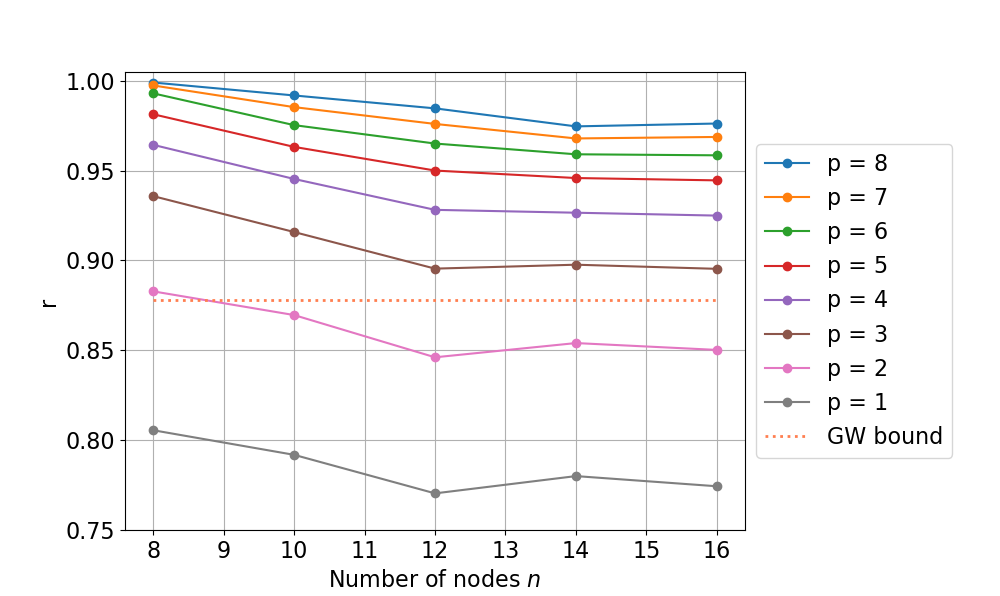
\includegraphics[width=0.85\textwidth]{figures/interp/INT_n_dependence.png}
		\captionsetup{justification=centering}
		\caption{INTERP $\qquad$ $\qquad$}
		\label{fig:r-n_dependence}
	\end{subfigure}
	\begin{subfigure}[t]{0.38\textwidth}
		\centering
		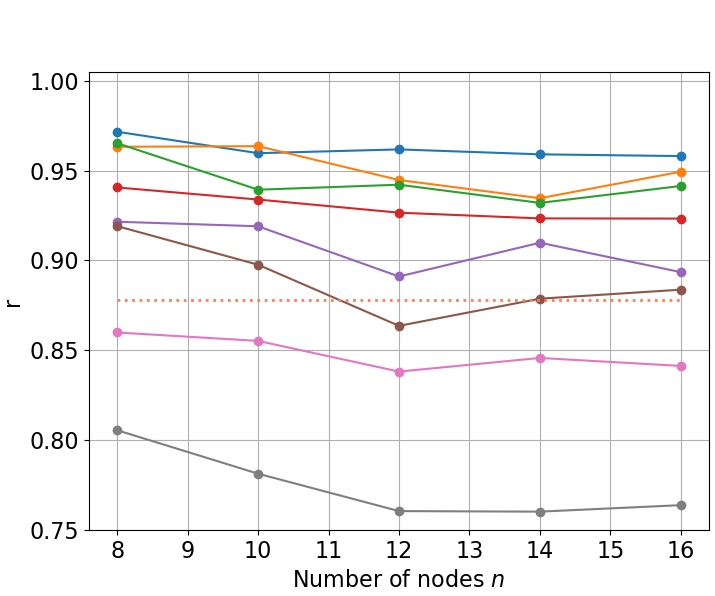
\includegraphics[width=\textwidth]{figures/RI/RI_n_dependence_3-regular_cut.png}
		\captionsetup{justification=centering}
		\caption{RI}
	\end{subfigure}
	\caption{Dependence of $r$ on $n$ on 20 randomly generated unweighted 3-regular graphs using both pyQuil INTERP (a) as well as pyQuil RI (b).  In both figures the lower bound of $0.878$ for the GW-algorithm is included.}
\end{figure}


The number of function evaluations necessary for parameter determination was also analyzed, see Figure \ref{fig:n_evals-3-regular}. The numerical results suggest that indeed the method is polynomial in $p$. For 3-regular graphs it was found that the necessary number of function evaluations was less than the number of function evaluations required for finding parameters for unweighted graphs.
\begin{figure}[H]
	\begin{subfigure}[t]{0.5\textwidth}
		\centering
		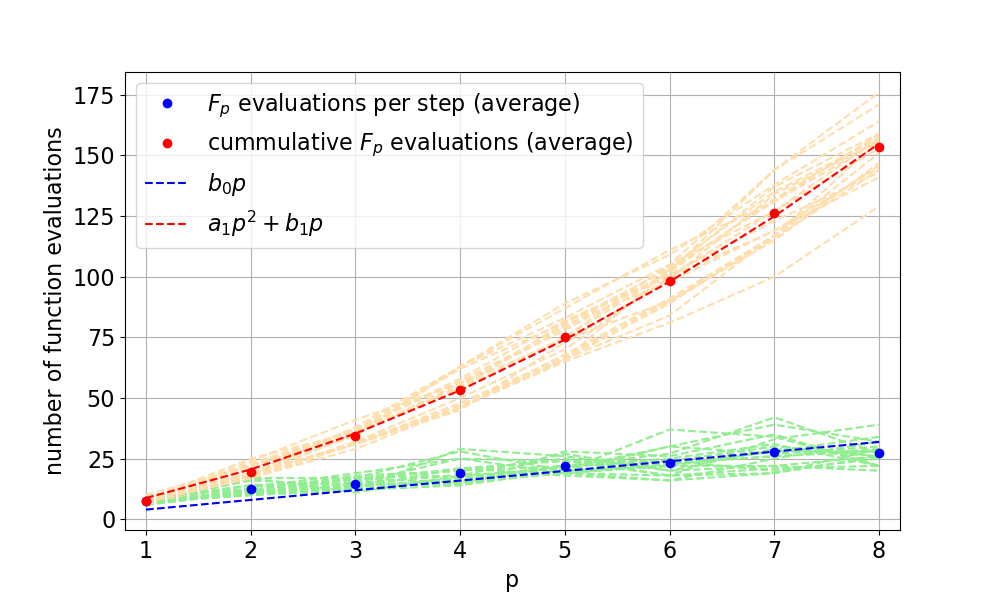
\includegraphics[width=\textwidth]{figures/interp/function_evaluations_16-nodal_unweighted.png}
		\captionsetup{justification=centering}
		\caption{Unweighted}
	\end{subfigure}
	\begin{subfigure}[t]{0.5\textwidth}
		\centering
		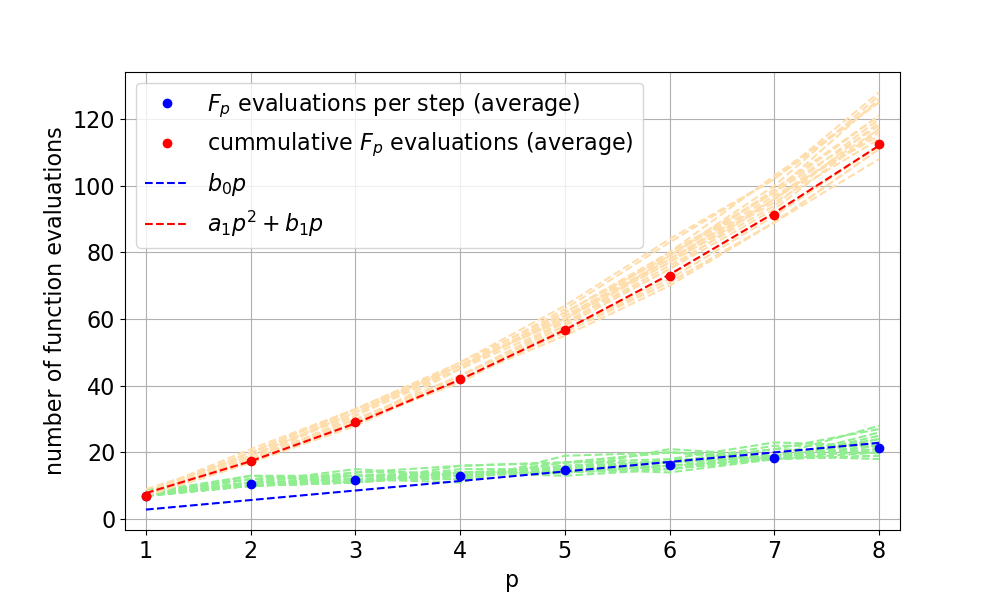
\includegraphics[width=\textwidth]{figures/interp/function_evaluations_16-nodal_weighted.png}
		\captionsetup{justification=centering}
		\caption{Weighted}
	\end{subfigure}
	\caption{Number of function evaluations necessary for parameter optimization in INTERP for 20 instances of 16-nodal 3-regular graphs. Both unweighted (a) and weighted (b). The fit parameters for the mean of the unweighted graphs are $b_0 = 4.0 \pm 0.2, a_1 = 1.52 \pm 0.05, b_1 = 7.2 \pm 0.3$. For the mean of the weighted graph the fitparameters found were $b_0 = 2.8 \pm 0.2, a_1 = 0.89 \pm 0.02, b_1 = 6.9 \pm 0.1$.}	
	\label{fig:n_evals-3-regular}
\end{figure}

\section{Erd\"os-R\'enyi graphs}
I also examined the performance of QAOA on Erd\"os-R\'enyi (ER) graphs with edge probability 0.50 and 0.75, abbreviated as ER-0.50 and ER-0.75 respectively. For graphs of this ensemble we find that the dependence of the fractional error acts similar to that of weighted 3-regular graphs as it also decreases exponentially with the square root of $p$, see Figure \ref{fig:fom-ER}.

\begin{figure}[H]
	\centering
	\begin{subfigure}[t]{0.48\textwidth}
		\centering
		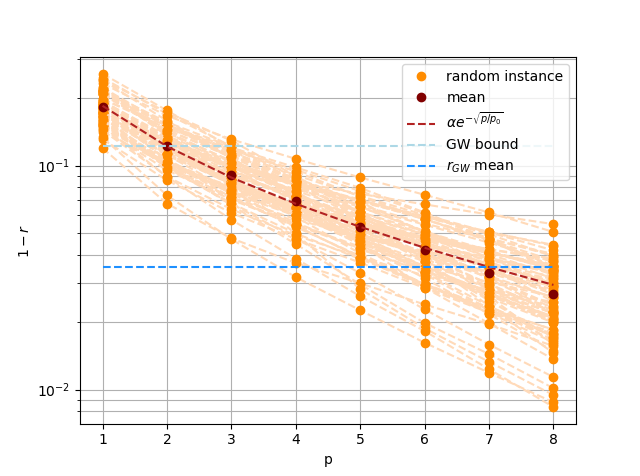
\includegraphics[width=\textwidth]{figures/interp/fom_er050.png}
		\caption{Fractional error $1-r$ for ER-0.50 graphs (20 instances). The fit parameters are $\alpha = 0.51 \pm 0.01$ and $p_0 = 0.99 \pm 0.03$.}
	\end{subfigure}%
	~
	\begin{subfigure}[t]{0.48\textwidth}
		\centering
		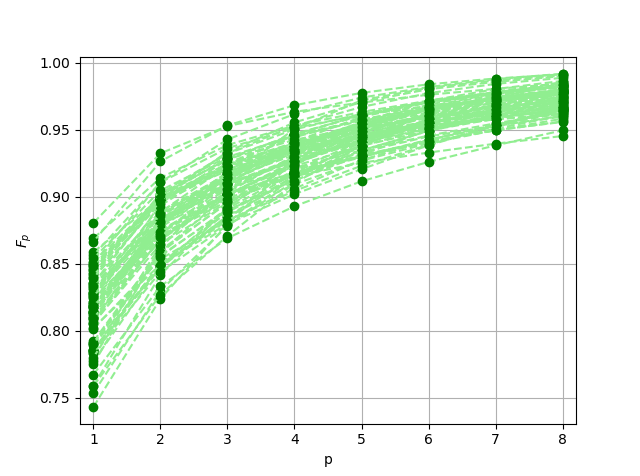
\includegraphics[width=\textwidth]{figures/interp/r_er050.png}
		\caption{Figure of merit $r$ for ER-0.50 graphs (20 instances).}
	\end{subfigure}%
	\\
	\begin{subfigure}[t]{0.48\textwidth}
		\centering
		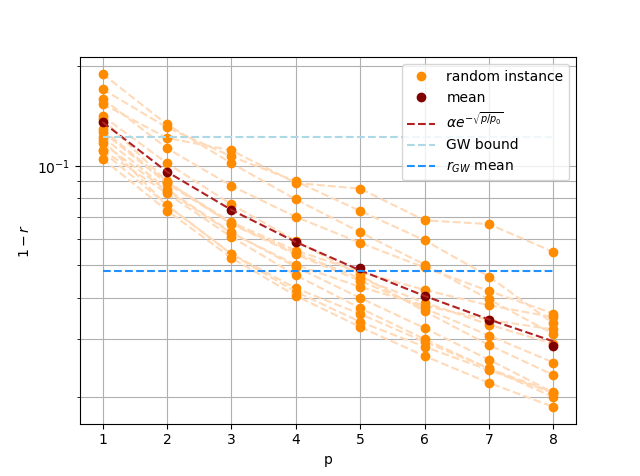
\includegraphics[width=\textwidth]{figures/interp/fom_er075.png}
		\caption{Fractional error $1-r$ for ER-0.75 graphs (10 instances). The fit parameters are $\alpha = 0.164 \pm 0.007$ and $p_0 = 4.1 \pm 0.3$}
	\end{subfigure}
	~
	\begin{subfigure}[t]{0.48\textwidth}
		\centering
		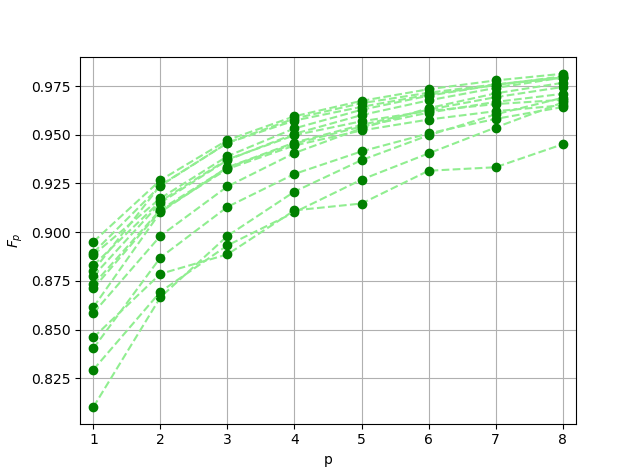
\includegraphics[width=\textwidth]{figures/interp/r_er075.png}
		\caption{Figure of merit $r$ for ER-0.75 graphs (10 instances)}
	\end{subfigure}%
	\caption{The fractional error and figure of merit for 12 nodal graphs of the Erd\"os-R\'enyi ensemble with edge probabilities 0.50 (a), (b) and 0.75 (c), (d) using the INTERP method for finding the parameters.}
	\label{fig:fom-ER}
\end{figure}

The dependence of $r$ on the number of nodes $n$ for the Erd\"os-R\'enyi graphs is shown in Figure \ref{fig:r-n_dependence_ER}. Again, we observe a general decreasing pattern in $r$ with $n$ from $p=4$ onwards. 

\begin{figure}[H]
	\begin{subfigure}[t]{0.6\textwidth}
		\centering
		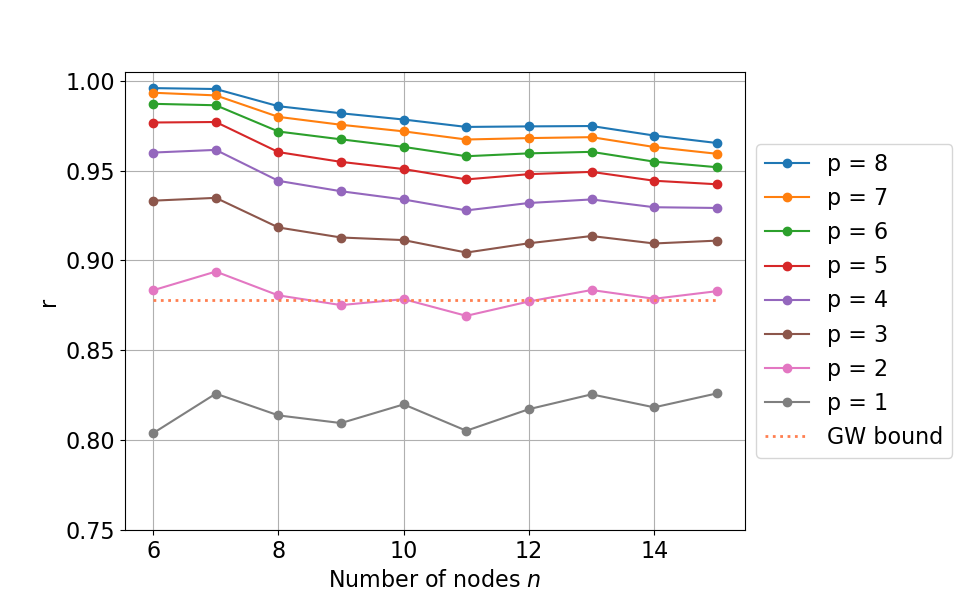
\includegraphics[width=0.85\textwidth]{figures/interp/INT_n_dependence_ER050.png}
		\captionsetup{justification=centering}
		\caption{ER-0.50}
		
	\end{subfigure}
	\begin{subfigure}[t]{0.4\textwidth}
		\centering
		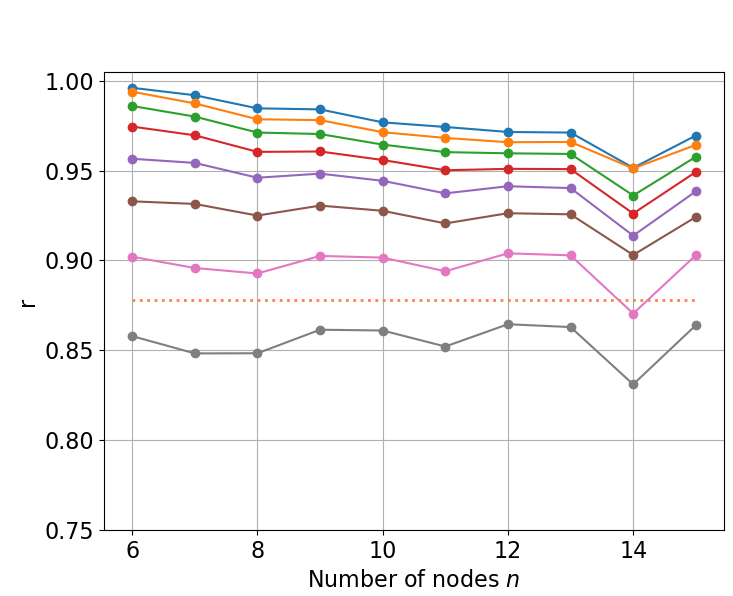
\includegraphics[width=\textwidth]{figures/interp/INT_n_dependence_ER075.png}
		\captionsetup{justification=centering}
		\caption{ER-0.75}
	\end{subfigure}
	\caption{Dependence of $r$ on $n$ on randomly generated unweighted ER graphs with edge probability 0.50 (a) as well 0.75 (b). In both figures the lower bound of $0.878$ for the GW-algorithm is included.}
	\label{fig:r-n_dependence_ER}
\end{figure}

The number of function evaluations for parameter determination is shown in figure \ref{fig:function-evaluations-ER}. We again observe that the method is polynomial in $p$. There seems to be no significant difference in the number of required function evaluations when comparing ER-0.50 and ER-0.75 graphs.
\begin{figure}[H]
	\centering
	\begin{subfigure}[t]{0.48\textwidth}
		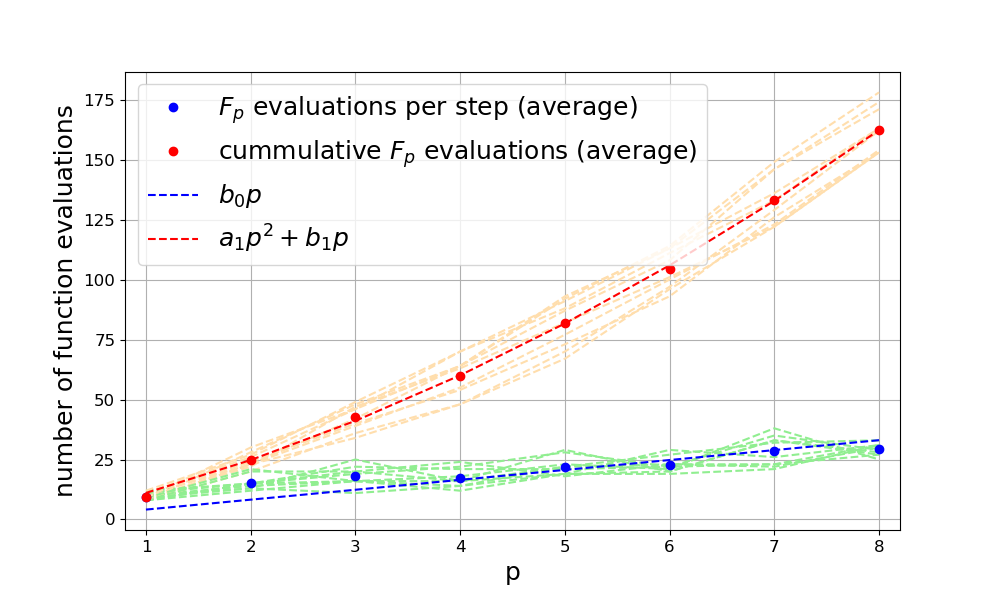
\includegraphics[width=\textwidth]{figures/interp/function_evaluations_15-nodal_ER050.png}
		\caption{15 nodal ER-0.50 graphs (20 instances)}
	\end{subfigure}
	\begin{subfigure}[t]{0.48\textwidth}
		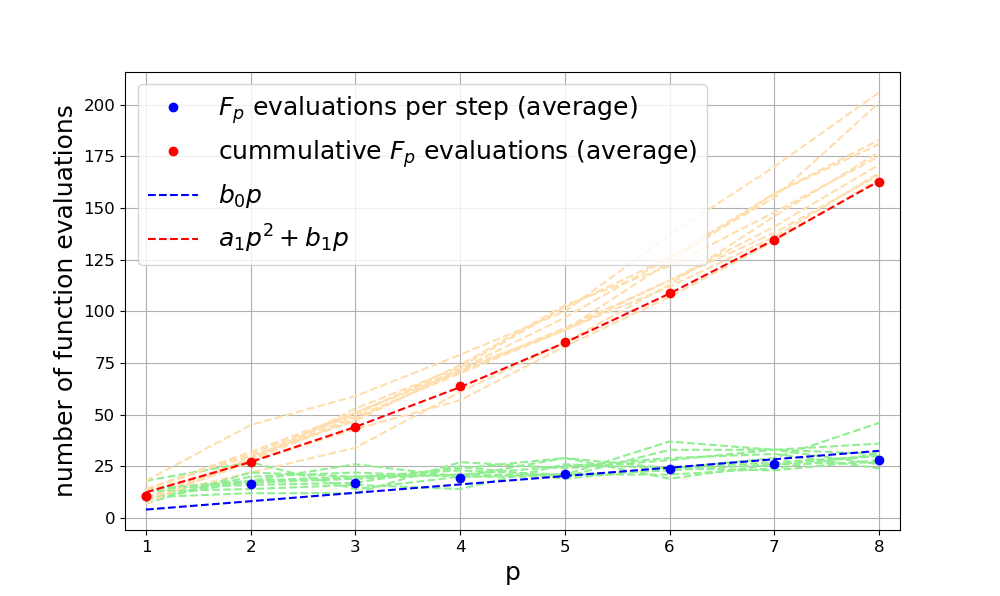
\includegraphics[width=\textwidth]{figures/interp/function_evaluations_15-nodal_ER075.png}
		\caption{15 nodal ER-0.75 graphs (10 instances)}
	\end{subfigure}
	\caption{Number of $F_p$ function evaluations necessary for the INTERP method to converge on ER graphs with 15 nodes. (a) 20 instances with edge probability 0.5 and fit parameters $b_0 = 4.1\pm0.3$ and $a_1=1.32 \pm 0.04, b_1 = 9.7\pm0.3$ (b) 10 instances with edge probability 0.75 and fit parameters $b_0 = 4.5\pm0.4$ and $a_1=1.25 \pm 0.03, b_1 = 12.4\pm0.2$. }
	\label{fig:function-evaluations-ER}
\end{figure}

\section{Cyclic graphs}
In the original QAOA paper \cite{FGG14}, an analytical expression for $F_p$ was derived by analyzing the contribution of subgraphs of size $p$ to the expectation value. As the graphs are cyclic, for $p<n/2$ there is only one type of subgraph, namely, a linear array of nodes. After maximizing the function numerically for $p=1,2,3,4,5$ and $6$ it was conjectured that for cyclic graphs one finds
\begin{equation}
\max_{\gambe}F_p = M_p = n\frac{2p+1}{2p+2}
\label{eq:cyclic-conjecture}
\end{equation}
for all $p < n/2$. To test this conjecture, I applied the pyQuil INTERP method to cyclic graphs. The $F_p$ values found by this method is shown in Figure \ref{fig:cyclic-conjecture}.

\begin{figure}[H]
	\centering
	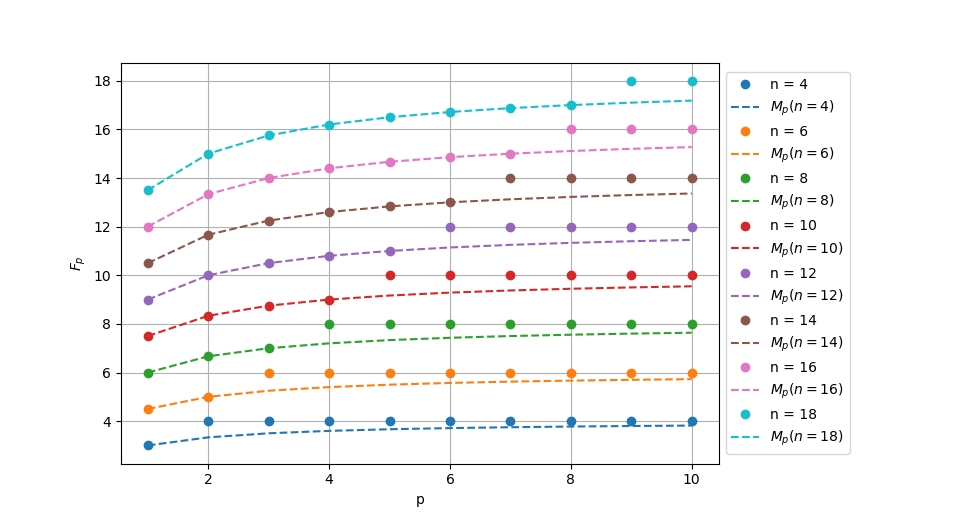
\includegraphics[width=0.9\textwidth]{figures/interp/cyclic_conjecture.png}
	\caption{The expectation value $F_p$ using the pyQuil INTERP method, for cyclic graphs with an even number of nodes $n$. The dots indicate the actual $F_p$ values from 1024 samples of the state. The dashed lines indicates the $M_p(n)$ values from Equation \eqref{eq:cyclic-conjecture} for various $n$ as a function of $p$.}
	\label{fig:cyclic-conjecture}
\end{figure}
It is noteworthy that for $p<n/2$ we indeed find that $M_p$ bounds $F_p$, and using the pyQuil INTERP method we attain that maximum $M_p$ with high precision. Beyond that, for $p \geq n/2$, the expectation value $F_p$ jumps to the facinity of the optimum value, namely $C_{\max} = n$, meaning $|\gambe\rangle$ is a groundstate of $-H_C$. 

In Figure \ref{fig:r-cyclic} the figure of merit $r$ is shown for cyclic graphs. As can be seen, there is a stark contrast between cyclic graphs with an even number of nodes, and an odd number of nodes. This is because the latter group has more partitions that are optimal as there has to be one neighbouring pair that are on the same side of the partition. Cyclic groups with an even number of nodes simply have one groundstate partitions, up to $\mathbb{Z}_2$ symmetry, namely an alternating bit string. This means that the groundstate of $-H_C$ has a higher degeneracy and thus the parametrized state $|\gambe\rangle$ naturally overlaps more with the groundstate.

\begin{figure}[H]
	\centering
	
	\begin{subfigure}[t]{0.5\textwidth}
		\centering
		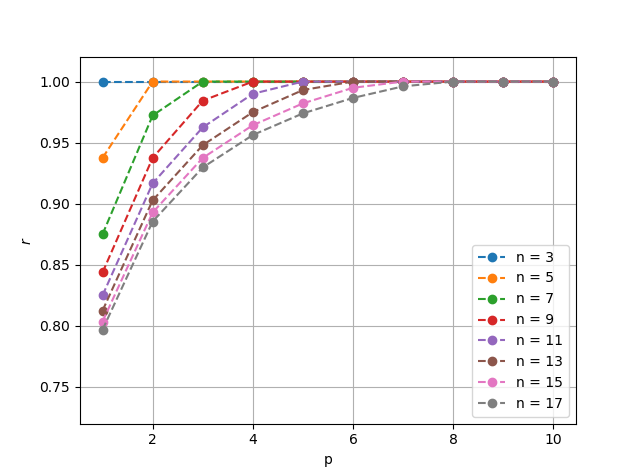
\includegraphics[width=\textwidth]{figures/interp/r_cyclic_odd.png}
		\caption{Odd $n$ where $C_{\max} = n-1$}
	\end{subfigure}%
	~ 
	\begin{subfigure}[t]{0.5\textwidth}
		\centering
		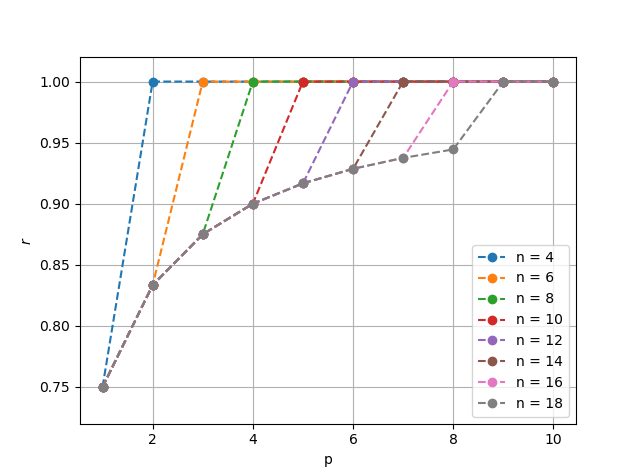
\includegraphics[width=\textwidth]{figures/interp/r_cyclic_even.png}
		\caption{Even $n$ where $C_{\max} = n$}
	\end{subfigure}
	\caption{Figure of merit $r$ for cyclic graphs of sizes $n= 2, \dots , 18$. The values for $F_p$ are acquired using the angles obtained using the pyQuil INTERP method.}
	\label{fig:r-cyclic}
\end{figure}

